\subsection{Definition of State Machines}
A state machine in the FW Profile consists of the following elements:

\begin{fw_itemize}
\item One \emph{initial pseudo-state}
\item One or more \emph{states}
\item One or more \emph{state transitions}
\item Zero or more \emph{choice pseudo-states}
\item Zero or more \emph{final pseudo-states}
\item Two \emph{execution counters}
\end{fw_itemize}

The \emph{initial pseudo-state} is characterized by one transition which has the initial pseudo-state as its source and has either a state or a choice pseudo-state as its target.

A \emph{state} is characterized by the following elements:

\begin{fw_itemize}
\item Zero or more \emph{entry actions}
\item Zero or more \emph{do actions}
\item Zero or more \emph{exit actions}
\item Zero or one \emph{embedded state machine}
\item One or more \emph{incoming transitions} 
\item Zero or more \emph{outgoing transitions}
\end{fw_itemize}

The state actions represent behaviour which is not decomposed further within the state machine. Actions' behaviour can be defined using natural 
language or some formalism (e.g. an action language). An embedded state machine is a state machine that is embedded within the state. Embedded state 
machines are defined in the same way and have the same behaviour as other FW Profile state machines. An incoming transition is a state transition that 
has the state as its target. An outgoing transition is a state transition that has the state as its source. 

A \emph{state transition} is characterized by the following elements:

\begin{fw_itemize}
\item One \emph{transition source}
\item One \emph{transition target} (or \emph{transition destination})
\item Zero or one \emph{transition trigger} (or \emph{transition command})
\item Zero or one \emph{transition guard}
\item Zero or more \emph{transition actions}
\end{fw_itemize}

The transition source and the transition target are either a state or a pseudo-state. The transition trigger is the command that triggers the execution 
of the transition. A transition guard is a specification that evaluates either to TRUE or to FALSE and has no side effects. Absence of a guard is equivalent to a guard which always evaluates to TRUE. A transition action represents 
behaviour which is not decomposed further within the state machine. A transition action behaviour can be defined using natural language or some formalism 
(e.g. an action language). Transition commands may carry parameters and may return values. The parameters and return values are not defined further by the 
FW Profile. They represent parameters that are passed to the actions and values which are returned by them. 

A \emph{choice pseudo-state} is characterized by the following elements:

\begin{fw_itemize}
\item One or more \emph{incoming transitions} 
\item One or more \emph{outgoing transitions}
\end{fw_itemize}

An incoming transition is a state transition that has the choice pseudo-state as its target. An outgoing transition is a state transition that has the 
choice pseudo-state as its source.

The \emph{final pseudo-state} is characterized by one or more incoming transitions (namely state transitions that have the final pseudo-state as their target). 
Note that all final pseudo-states are equivalent and therefore it would be legitimate to allow only one single final pseudo-state. The option to have more 
than one is introduced as a matter of convenience.

The \emph{execution counters} are unsigned integers which are characterized by their value.
The first execution counter is called the \emph{State Machine Execution Counter} and the second one
is called the \emph{State Execution Counter}.

The following syntactical constraints apply to the definition of the state machine elements:

\begin{fw_itemize}
\item{\textbf{C1}}: The same pseudo-state cannot be both source and target for a transition;
\item{\textbf{C2}}: The source and target of a transition cannot both be choice pseudo-states;
\item{\textbf{C3}}: The transition that has the initial pseudo-state as source can have neither a guard nor a trigger;
\item{\textbf{C4}}: This constraint has been deleted;
\item{\textbf{C5}}: Transitions that have a choice pseudo-state as source cannot have a transition trigger;
\item{\textbf{C6}}: This constraint has been deleted;
\item{\textbf{C7}}: Transitions that have a state as a source must have a transition command;
\item{\textbf{C8}}: Transitions can only link states and/or pseudo-states that belong to the same state machine.
\end{fw_itemize}

The last constraint implies that transitions from an outer state machines to an embedded state machines or vice-versa are not allowed. Note, however, 
that the same transition command may trigger a transition both in an outer state machine and in one of its embedded state machine. 

The following dynamical constraints must be satisfied when a state transition is executed: 

\begin{fw_itemize}
\item{\textbf{D1}}: Among the outgoing transitions from a choice pseudo-state, at least one must have a guard that evaluates to true.
\item{\textbf{D2}}: Transition guards must be free of side effects: their evaluation cannot change the state of the host application.
\item{\textbf{D3}}. The state actions (entry, do, and exit actions) and the transition actions and guards must execute
in zero logical execution time (i.e. on an infinitely fast processor and in the absence of pre-emption or blocking, 
they must execute in zero time).
\end{fw_itemize}

The last constraint implies that the behaviour encapsulated by actions and guards is
constrained to be \emph{purely functional}. In practice, this means that actions and guards cannot
include time-dependent behaviour or behaviour that depends on synchronization with other
flows of executions.

One type of transition command the \emph{Execute} command has a special status in that it triggers the execution of the current state's do-action. 
The Execute command models the situation (common in embedded control systems) of a cyclical scheduler periodically triggering 
an application and advancing its execution.

As a matter of terminology, when a state machine is sent the Execute command, the state
machine is said to be \emph{executed}.

The execution counters of a state machine count the number of times the state machine has
been executed (one counts the number of times the state machine has been executed since it 
was started and the other counts the number of times the state machine has been executed
since its current state was entered). Since state machines will often be executed periodically,
the execution counters can serve as proxies for measuring the elapsing of time.


\subsection{State Machine Behaviour}
Three operations may be performed on a state machine: 
(a) the state machine may be \emph{started}; 
(b) the state machine may be \emph{sent a transition command}; or 
(c) the state machine may be \emph{stopped}. 
State machines are purely reactive: they wait for one of these three operations to be performed 
upon them and they only execute some behaviour in response to one of these operations. 

A state machine can be either in a defined state or in an undefined state. 
A state machine is in a defined state from the time it has completed the 
transition out of its initial pseudo-state to the time it has either completed the transition into one of its final pseudo-states or has been stopped.

When a state machine is in a defined state, it has a \emph{current state}. The current state is one of the states of the state machine.

When a state machine is started, the following behaviour is executed:

\begin{fw_enumerate}
\item If the state machine is in a defined state, then no further action is taken.
\item If the state machine is in an undefined state, then its execution counters are reset
and the action associated to the transition
out of its initial pseudo-state is executed. If several transition actions are present, they
are executed in the order in which they are listed.
\item If the destination of the transition out of the initial pseudo-state is a choice pseudo-
state, then the guards of the outgoing transitions from the choice pseudo-state are
evaluated and the actions associated to the transition with a guard evaluating to true is
executed. If several transition actions are present, they are executed in the order in
which they are listed.
\item If the destination of the transition out of the initial pseudo-state is a state, then the
current state of the state machine is set equal to that state.
\item If the destination of the transition out of the initial pseudo-state is a choice pseudo-
state and if the selected transition out of the choice pseudo-state has a state as a target,
then the current state of the state machine is set equal to that target state.
\item The entry action of the current state is executed. If several entry actions are present,
they are executed in the order in which they are listed.
\item If the current state has an embedded state machine, then the embedded state machine is
started.
\item If the destination of the transition out of the initial pseudo-state is a choice pseudo-
state and if the selected transition out of the choice pseudo-state has the final pseudo-
state as a target, then the state machine remains in an undefined state.
\end{fw_enumerate}

With reference to point 3, it is noted that at least one of the guards on the outgoing transitions from a choice pseudo-state is guaranteed to be true 
because of constraint D1 in the previous section.

When a state machine is stopped, the following behaviour is executed:

\begin{fw_enumerate}
\item If the state machine is in an undefined state, no further action is taken.
\item If the state machine is in a defined state and its current state has an embedded state machine, the embedded state machine is stopped.
\item The exit action of the current state is executed. If several exit actions are present, they are executed in the order in which they are listed.
\item The state machine is set to an undefined state.
\end{fw_enumerate}

The logic of the start and stop commands for state machines is shown in Figure \ref{fig:logicStartStopCmdSM} as two activity diagrams.

\begin{figure}[ht]
 \centering
 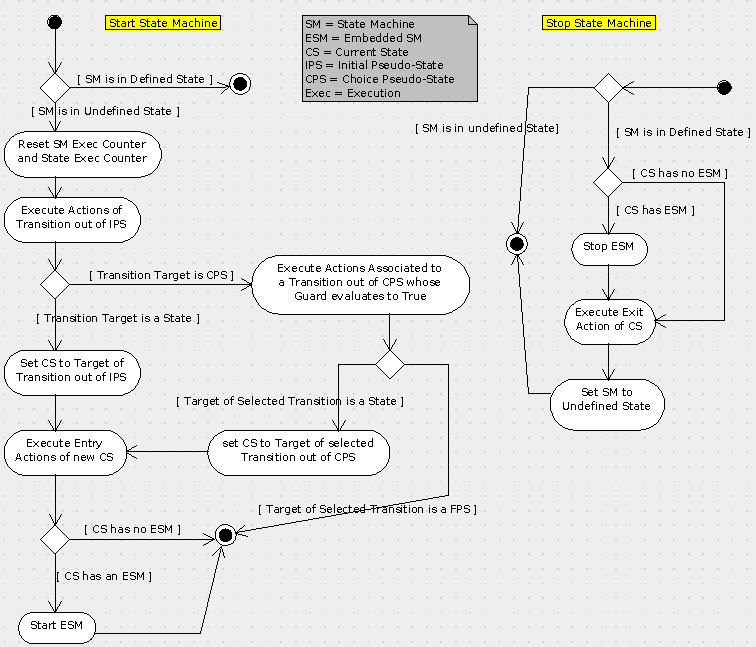
\includegraphics[scale=0.415,keepaspectratio=true]{SM_StartStop.png}
 % SMD.png: 474x227 pixel, 72dpi, 16.72x8.01 cm, bb=0 0 474 227
 \caption{Logic for the Start and Stop Commands to a State Machine}
 \label{fig:logicStartStopCmdSM}
\end{figure}

When a transition command T is sent to a state machine S, then the following behaviour is executed:

\begin{fw_enumerate}
\item If S is in an undefined state, then no further action is taken.
\item If T is the Execute command, then the execution counters of the state machine are
incremented and the do-action associated to the current state of S is
executed. If several do-actions are present, they are executed in the order in which
they are listed.
\item If S is in a defined state and the current state of S has an embedded state machine SE,
then the transition command T is propagated to SE.
\item If there are no transitions from the current state of S that have T as their trigger, then
no further action is taken.
\item If there are one or more transitions from the current state of S that have T as their
trigger, then their guards are evaluated in sequence. The order of the evaluation is
undefined. The absence of a guard is equivalent to a guard that returns TRUE.
\item When the first transition is found whose guard evaluates to TRUE, then that transition
is executed.
\end{fw_enumerate}

The logic that governs the processing of a transition command by a state machine is shown in Figure \ref{fig:logicTransitionCmdSM} as an activity diagram. 
Note that this logic merely describes the circumstances under which a transition within a state machine is executed but it does not define the logic 
according to which the transition is executed. This is done below (see also Figure \ref{fig:execTransitionSM}).

\begin{figure}[ht]
 \centering
 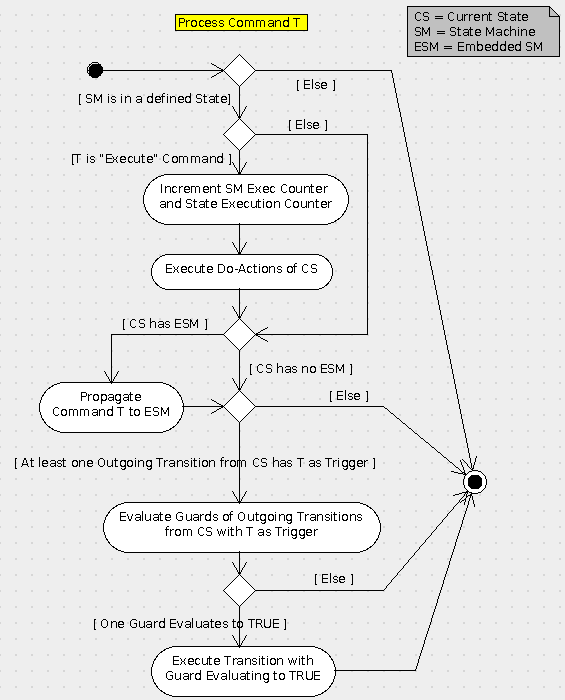
\includegraphics[scale=0.5,keepaspectratio=true]{SM_CmdProcessing.png}
 % SMD.png: 474x227 pixel, 72dpi, 16.72x8.01 cm, bb=0 0 474 227
 \caption{Logic for Processing Transition Commands by a State Machine}
 \label{fig:logicTransitionCmdSM}
\end{figure}

When a transition is executed, then the following behaviour is executed:

\begin{fw_enumerate}
\item If the source state of the transition is a state and that state has an embedded state
machine, then the embedded state machine is stopped.
\item If the source state of the transition is a state, then the exit action associated to the
source state is executed. If several exit actions are present, they are executed in the
order in which they are listed.
\item The transition action associated to the transition is executed. If several transition
actions are present, they are executed in the order in which they are listed.
\item If the target of the transition is a choice pseudo-state, then the guards of the out-going
transitions from the choice pseudo-state are evaluated in sequence until one is found
that evaluates to true and that transition is executed.
\item If the target of the transition is a final pseudo-state, then the state machine is set to an
undefined state and no further action is taken.
\item If the target state of the transition is a state, then the current state of the state machine
is updated to be equal to the target state of the transition and the state execution counter is
reset.
\item If the target state of the transition is a state, then the entry action of the target state is
executed. If several entry actions are present, they are executed in the order in which
they are listed.
\item If the target state of the transition is a state and that state has an embedded state
machine, then the embedded state machine is started.
\end{fw_enumerate}

With reference to point 4, it is noted that at least one of the guards on the outgoing transitions from a choice pseudo-state is guaranteed to be true 
because of constraint \textbf{D1} in the previous section.
The logic according to which a transition is executed is shown as an activity diagram in Figure \ref{fig:execTransitionSM}. Note that this logic is called up 
by the logic shown in the activity diagram of Figure \ref{fig:logicTransitionCmdSM}.

\begin{figure}[ht]
 \centering
 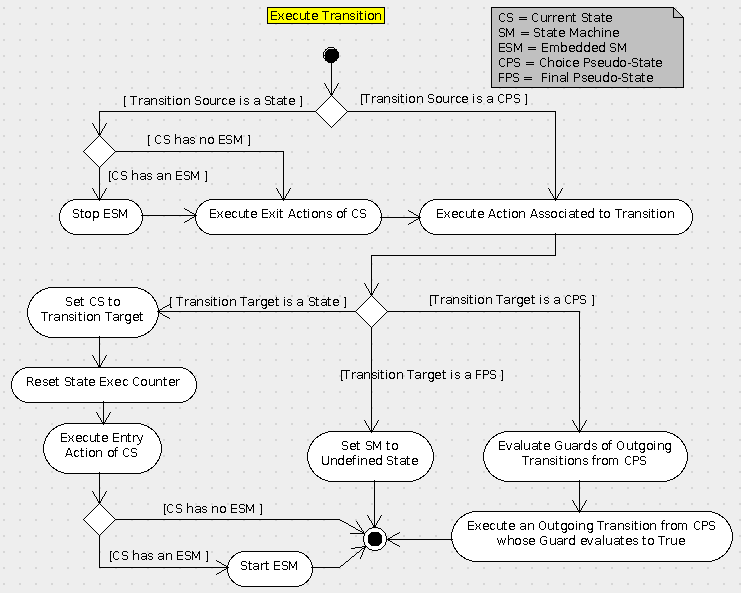
\includegraphics[scale=0.45,keepaspectratio=true]{SM_TransitionExecution.png}
 % SMD.png: 474x227 pixel, 72dpi, 16.72x8.01 cm, bb=0 0 474 227
 \caption{Logic for Executing Transitions in a State Machine}
 \label{fig:execTransitionSM}
\end{figure}

Transition commands may carry parameters. These parameters may be passed to any of the state or transition actions that are executed as part of 
the processing of the transition command.

The execution of the various actions associated to the three state machine operations is performed in sequence: an action is executed only when 
the previous one has completed. Note that, since state and transition actions are constrained to execute in zero logical execution time, 
the execution of a state machine operation will also execute in zero logical execution time.  

Transition commands arrive and are processed in sequence. A new command can only arrive and be processed by a state machine when the previous one has 
been fully processed. State machines have no queues to buffer incoming transition commands.

The above rule in particular implies that transition commands cannot be nested, namely the processing of a transition command by a state machine 
cannot result in a new command being sent to the same state machine (nesting rule).

As an example where the nesting rule would be violated, consider the following situation. A first transition command is sent to state machine A that 
triggers a transition from state A1 to state A2. The entry action of state A2 sends a second transition command to state machine A. 

As a second example of violation of the nesting rule, consider  a  transition command that is sent to state machine A that triggers a transition 
from state A1 to state A2. The entry action of state A2 sends a new transition command to state machine B. State machine B, as part of its processing 
of this command, sends a new transition command to state machine A.

Forwarding of transition commands from one state machine A to another state machine B is instead allowed provided that neither of the two state machines 
is embedded in the other one. 

Forwarding of transition commands from an embedded state machine to its embedding state machine or vice-versa is forbidden. This restriction helps 
to avoid the ambiguities that would arise when, for instance, the entry action of a state in an embedded state machine triggers a transition in 
the embedding state machine.

\subsection{UML 2 Compliance}
The state machine model offered by the FW Profile complies with the UML 2 state machine
model in the sense that the elements of the state machine concept of the FW Profile and their
semantics can be mapped in an obvious way to a subset of the elements of the state machine
concept of UML 2 with the following provisos:

\begin{fw_itemize}
\item The semantics of choice pseudo-states in the FW Profiles subsumes that of junction pseudo-states
in UML2. Thus, in the FW Profile, choice pseudo-states can also be used to join together incoming
transition flows.
\item The execution counters are specific to the FW Profile. They have been introduced as a
substitute for the concept of time (which does not exist in the FW Profile State Machines) in
the sense that, if state machines are executed periodically, then the value of their execution 
counters is proportional to the time elapsed since the state machine was started (State Machine
Execution Counter) or since the current state was entered (State Execution Counter). 
\end{fw_itemize}

It should be emphasized that the state machine model proposed by the FW Profile is far more
restrictive than that supported by UML 2. This is because the FW Profile uses state machines
to model purely functional (non-time-related) behaviour.

